
\begin{frame}{Equações Diferenciais Ordinárias (EDOs)}
    \begin{itemize}
        \item Usadas para estudar o comportamento populacional ao longo do tempo;
        \item Diversas aplicações em várias áreas do conhecimento;
        \note[item]{Exemplos de uso de EDOs: medicina, neurociência, estudo do câncer.}
        \item Cada equação descreve a concentração de uma população diferente;
    \end{itemize}

    \begin{columns}
        \begin{column}{.4\textwidth}
            \begin{equation}
                \begin{array}{lr}
                    \frac{dN_1}{dt} = r_1.N_1(1 - W_{11}.N_1 - W_{21}.N_2)
                    \\
                    \\
                    \frac{dN_2}{dt} = r_2.N_2(1 - W_{22}.N_2 - W_{12}.N_1)
                \end{array}
            \end{equation}
        \end{column}

        \begin{column}{.6\textwidth}
            \begin{figure}
                \centering
                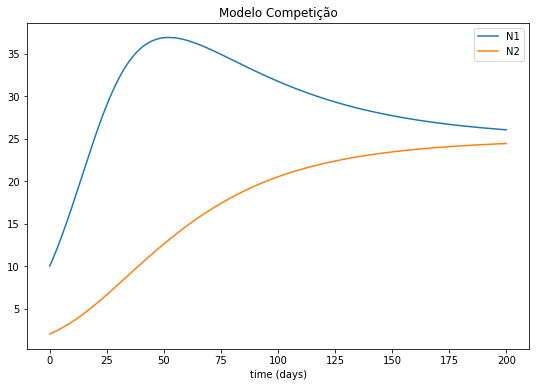
\includegraphics[height=.7\textheight]{beamerthemesrc/images/ode}
            \end{figure}
        \end{column}
    \end{columns}
\end{frame}

\begin{frame}{EDO — Modelo Predador-Presa}
    Um modelo clássico da literatura é o modelo Predador-Presa. Este modelo descreve o comportamento de duas populações, $H$ e $P$, que possuem uma uma relação de predação entre si. 

    \begin{columns}
        \begin{column}{.3\textwidth}
            \begin{equation}\label{eq:predadorpresa}
                \begin{array}{lr}
                    \frac{dH}{dt} = r.H - a.H.P
                    \\
                    \\
                    \frac{dP}{dt} = b.H.P - m.P
                \end{array}
            \end{equation}
        \end{column}
        \begin{column}{.6\textwidth}
            Na equação, temos que
            \[
            \begin{array}{lr}
                H & \text{Presa}\\
                P & \text{Predador}\\
                r & \text{Taxa de reprodução da presa}\\
                m & \text{Taxa de mortalidade dos predadores}\\
                a & \text{Taxa de predação}\\
                b & \text{Taxa de reprodução dos predadores}\\
                \end{array}.
            \]
        \end{column}
    \end{columns}

    \note[item]{
        Neste modelo, temos os seguintes processos sendo modelados: 
        \begin{itemize}
            \item Reprodução das presas ($r.H$);
            \item Predação ($a.H.P$);
            \item Reprodução dos predadores ($b.H.P$);
            \item Morte dos predadores ($m.P$). 
        \end{itemize}
    }
    \note[item]{
        Termos de replicação, predação e morte como os vistos neste modelo são muito comuns. Estes termos são construídos com base no princípio da Lei de Ação de Massas, que diz que ``O número de interações entre duas partículas depende da concentração de ambas.''
    }
\end{frame}

\begin{frame}{Programação visual}
    \begin{itemize}
        \item É uma maneira do usuário programar a máquina por meio de elementos gráficos que abstraem instruções do computador.
        \item Os elementos podem representar múltiplas operações por vez, com o objetivo de facilitar a programação.
        \item Exemplos: GRAIL, Scratch, Logisim, Blender. 
        \note[item]{A linguagem GRAIL foi desenvolvida junto a uma tela sensível ao toque e uma \textit{stylus}}
        \item Um exemplo comum de aplicação envolve editores baseados em nós, que representam operações complexas de forma natural, combinando um conjunto de entradas para gerar uma ou mais saídas.
    \end{itemize}
\end{frame}

\begin{frame}{Geração de código}
    \begin{itemize}
        \item Recebe como entrada uma Representação Intermediária (RI) e gera como saída um código na linguagem alvo (por exemplo, Python).
        \item Aplicações da RI: 
        \begin{itemize}
            \item Separar o \textit{front-end} do \textit{back-end};
            \item Permitir que sejam realizadas otimizações independente de máquina ou otimizações independente da linguagem alvo; 
            \item Facilitar a tradução e geração do código alvo.
        \end{itemize}
        \item Exemplo: LLVM IR, usada originalmente para compilar códigos em C/C++ pelo Clang, e agora também usada na compilação de códigos em Rust.
    \end{itemize}    
\end{frame}

\begin{frame}{Geração de código baseada em \textit{templates}}
    \begin{itemize}
        \item Um \textit{template} é um esqueleto (uma estrutura) que serve de referência para todo o processo de geração de código.
        \item Em sua essência, \textit{templates} são arquivos com marcadores especiais que podem ser substituídos por outros valores dinamicamente.
        \item A presença de estruturas de controle de fluxo como condicionais e laços de repetição permitem a escrita de \textit{templates} legíveis e de fácil manutenção.
    \end{itemize}
\end{frame}

\begin{frame}[fragile]{Geração de código baseada em \textit{templates}}
    \begin{minted}{python}
    def system(t: np.float64, y: np.ndarray, *constants) -> np.ndarray:
        
            {{- arg.name }},  = y

        
        
            {{- arg.name }},  = constants
        

        
        
        d{{ pop.name }}_dt = {{ display_composite(comp) }}
        

        # ...
    \end{minted}
\end{frame}

% \begin{frame}{Ensino-aprendizagem de Modelagem Computacional}
%     \begin{figure}[h]
%         \centering
%         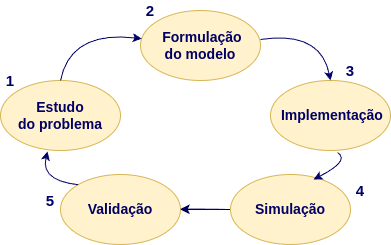
\includegraphics[scale=0.5]{contents/imgs/ciclo-modelagem.png} 
%         \caption{Visão geral do ciclo da modelagem.}
%         \label{fig:ciclo-modelagem}
%     \end{figure}
% \end{frame}
